\documentclass[11pt, oneside]{article}   	% use "amsart" instead of "article" for AMSLaTeX format
\usepackage{geometry}                		% See geometry.pdf to learn the layout options. There are lots.
\usepackage{textcomp}
\usepackage{hyperref}  % TODO: see page 94 of latex book
\geometry{letterpaper}                   		% ... or a4paper or a5paper or ... 
%\usepackage[parfill]{parskip}    		% Activate to begin paragraphs with an empty line rather than an indent
\usepackage{graphicx}				% Use pdf, png, jpg, or eps§ with pdflatex; use eps in DVI mode
								% TeX will automatically convert eps --> pdf in pdflatex		
\usepackage{amssymb}
\usepackage{relsize}

\title{CSCI 181 / E-181 Spring 2014 Practical 2 \\ 
{\large Kaggle Team "No Comment"}
}
\author{
  David Wihl\\
  \texttt{davidwihl@gmail.com}
  \and
  Zack Hendlin\\
  \texttt{zgh@mit.edu} 
}
%\date{}							% Activate to display a given date or no date

\begin{document}
\maketitle
\section*{Warm-Up}

%max g-forces eyeballs out is 12g eyeballs out http://www.gforces.net/human-tolerance-horizontal.html

%helmet tests on g forces http://www.smf.org/docs/articles/hic/Various_helmets_stds.pdf

\subsection*{Baseline}

\begin{figure}[h!] 
  \centering
  \scalebox{0.5}{{\large % GNUPLOT: LaTeX picture with Postscript
\begingroup
  \makeatletter
  \providecommand\color[2][]{%
    \GenericError{(gnuplot) \space\space\space\@spaces}{%
      Package color not loaded in conjunction with
      terminal option `colourtext'%
    }{See the gnuplot documentation for explanation.%
    }{Either use 'blacktext' in gnuplot or load the package
      color.sty in LaTeX.}%
    \renewcommand\color[2][]{}%
  }%
  \providecommand\includegraphics[2][]{%
    \GenericError{(gnuplot) \space\space\space\@spaces}{%
      Package graphicx or graphics not loaded%
    }{See the gnuplot documentation for explanation.%
    }{The gnuplot epslatex terminal needs graphicx.sty or graphics.sty.}%
    \renewcommand\includegraphics[2][]{}%
  }%
  \providecommand\rotatebox[2]{#2}%
  \@ifundefined{ifGPcolor}{%
    \newif\ifGPcolor
    \GPcolorfalse
  }{}%
  \@ifundefined{ifGPblacktext}{%
    \newif\ifGPblacktext
    \GPblacktexttrue
  }{}%
  % define a \g@addto@macro without @ in the name:
  \let\gplgaddtomacro\g@addto@macro
  % define empty templates for all commands taking text:
  \gdef\gplbacktext{}%
  \gdef\gplfronttext{}%
  \makeatother
  \ifGPblacktext
    % no textcolor at all
    \def\colorrgb#1{}%
    \def\colorgray#1{}%
  \else
    % gray or color?
    \ifGPcolor
      \def\colorrgb#1{\color[rgb]{#1}}%
      \def\colorgray#1{\color[gray]{#1}}%
      \expandafter\def\csname LTw\endcsname{\color{white}}%
      \expandafter\def\csname LTb\endcsname{\color{black}}%
      \expandafter\def\csname LTa\endcsname{\color{black}}%
      \expandafter\def\csname LT0\endcsname{\color[rgb]{1,0,0}}%
      \expandafter\def\csname LT1\endcsname{\color[rgb]{0,1,0}}%
      \expandafter\def\csname LT2\endcsname{\color[rgb]{0,0,1}}%
      \expandafter\def\csname LT3\endcsname{\color[rgb]{1,0,1}}%
      \expandafter\def\csname LT4\endcsname{\color[rgb]{0,1,1}}%
      \expandafter\def\csname LT5\endcsname{\color[rgb]{1,1,0}}%
      \expandafter\def\csname LT6\endcsname{\color[rgb]{0,0,0}}%
      \expandafter\def\csname LT7\endcsname{\color[rgb]{1,0.3,0}}%
      \expandafter\def\csname LT8\endcsname{\color[rgb]{0.5,0.5,0.5}}%
    \else
      % gray
      \def\colorrgb#1{\color{black}}%
      \def\colorgray#1{\color[gray]{#1}}%
      \expandafter\def\csname LTw\endcsname{\color{white}}%
      \expandafter\def\csname LTb\endcsname{\color{black}}%
      \expandafter\def\csname LTa\endcsname{\color{black}}%
      \expandafter\def\csname LT0\endcsname{\color{black}}%
      \expandafter\def\csname LT1\endcsname{\color{black}}%
      \expandafter\def\csname LT2\endcsname{\color{black}}%
      \expandafter\def\csname LT3\endcsname{\color{black}}%
      \expandafter\def\csname LT4\endcsname{\color{black}}%
      \expandafter\def\csname LT5\endcsname{\color{black}}%
      \expandafter\def\csname LT6\endcsname{\color{black}}%
      \expandafter\def\csname LT7\endcsname{\color{black}}%
      \expandafter\def\csname LT8\endcsname{\color{black}}%
    \fi
  \fi
  \setlength{\unitlength}{0.0500bp}%
  \begin{picture}(11520.00,8640.00)%
    \gplgaddtomacro\gplbacktext{%
      \colorrgb{0.00,0.00,0.00}%
      \put(860,640){\makebox(0,0)[r]{\strut{}-150}}%
      \colorrgb{0.00,0.00,0.00}%
      \put(860,2120){\makebox(0,0)[r]{\strut{}-100}}%
      \colorrgb{0.00,0.00,0.00}%
      \put(860,3600){\makebox(0,0)[r]{\strut{}-50}}%
      \colorrgb{0.00,0.00,0.00}%
      \put(860,5079){\makebox(0,0)[r]{\strut{}0}}%
      \colorrgb{0.00,0.00,0.00}%
      \put(860,6559){\makebox(0,0)[r]{\strut{}50}}%
      \colorrgb{0.00,0.00,0.00}%
      \put(860,8039){\makebox(0,0)[r]{\strut{}100}}%
      \colorrgb{0.00,0.00,0.00}%
      \put(980,440){\makebox(0,0){\strut{}-10}}%
      \colorrgb{0.00,0.00,0.00}%
      \put(2434,440){\makebox(0,0){\strut{}0}}%
      \colorrgb{0.00,0.00,0.00}%
      \put(3888,440){\makebox(0,0){\strut{}10}}%
      \colorrgb{0.00,0.00,0.00}%
      \put(5342,440){\makebox(0,0){\strut{}20}}%
      \colorrgb{0.00,0.00,0.00}%
      \put(6797,440){\makebox(0,0){\strut{}30}}%
      \colorrgb{0.00,0.00,0.00}%
      \put(8251,440){\makebox(0,0){\strut{}40}}%
      \colorrgb{0.00,0.00,0.00}%
      \put(9705,440){\makebox(0,0){\strut{}50}}%
      \colorrgb{0.00,0.00,0.00}%
      \put(11159,440){\makebox(0,0){\strut{}60}}%
      \colorrgb{0.00,0.00,0.00}%
      \put(160,4339){\rotatebox{90}{\makebox(0,0){\strut{}force on head (g)}}}%
      \colorrgb{0.00,0.00,0.00}%
      \put(6069,140){\makebox(0,0){\strut{}time since impact(ms)}}%
      \csname LTb\endcsname%
      \put(6069,8339){\makebox(0,0){\strut{}Linear Basis}}%
    }%
    \gplgaddtomacro\gplfronttext{%
      \csname LTb\endcsname%
      \put(10256,7876){\makebox(0,0)[r]{\strut{}Training Data}}%
      \csname LTb\endcsname%
      \put(10256,7676){\makebox(0,0)[r]{\strut{}Linear Basis}}%
    }%
    \gplbacktext
    \put(0,0){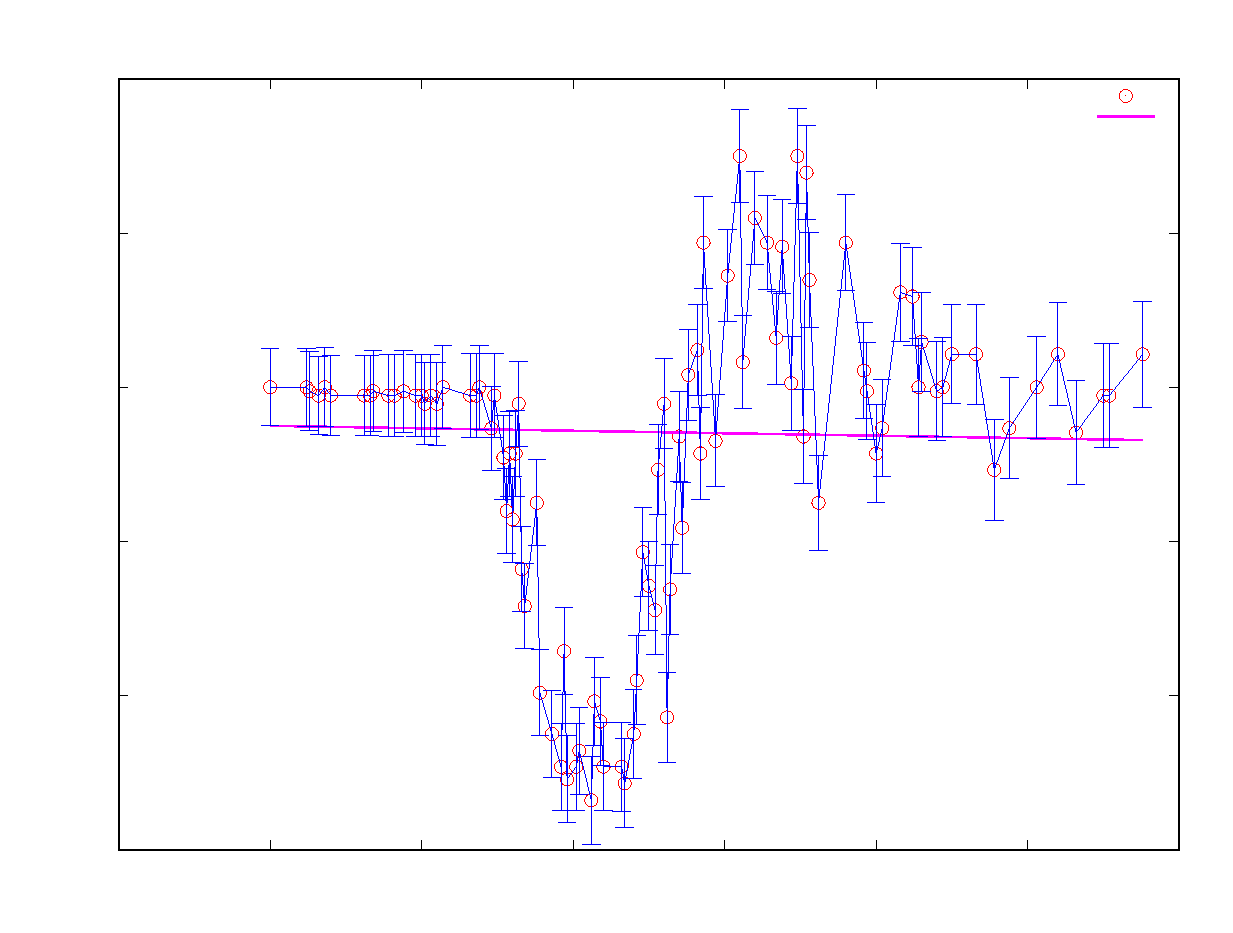
\includegraphics{linear}}%
    \gplfronttext
  \end{picture}%
\endgroup
}}
  \caption{Warmup: Linear Basis}
\end{figure}

As a baseline, we first created a simple linear gradient descent with a flat slope and intercept. 

We also used a polynomial basis, iterating with polynomials from $n^2$ up to $n^{12}$ and selecting the lowest error. Unsurprisingly, $n^{12}$ had the lowest error rate, but is likely highly overfit.

\begin{figure}[h!] 
  \centering
  \scalebox{0.5}{{\large % GNUPLOT: LaTeX picture with Postscript
\begingroup
  \makeatletter
  \providecommand\color[2][]{%
    \GenericError{(gnuplot) \space\space\space\@spaces}{%
      Package color not loaded in conjunction with
      terminal option `colourtext'%
    }{See the gnuplot documentation for explanation.%
    }{Either use 'blacktext' in gnuplot or load the package
      color.sty in LaTeX.}%
    \renewcommand\color[2][]{}%
  }%
  \providecommand\includegraphics[2][]{%
    \GenericError{(gnuplot) \space\space\space\@spaces}{%
      Package graphicx or graphics not loaded%
    }{See the gnuplot documentation for explanation.%
    }{The gnuplot epslatex terminal needs graphicx.sty or graphics.sty.}%
    \renewcommand\includegraphics[2][]{}%
  }%
  \providecommand\rotatebox[2]{#2}%
  \@ifundefined{ifGPcolor}{%
    \newif\ifGPcolor
    \GPcolorfalse
  }{}%
  \@ifundefined{ifGPblacktext}{%
    \newif\ifGPblacktext
    \GPblacktexttrue
  }{}%
  % define a \g@addto@macro without @ in the name:
  \let\gplgaddtomacro\g@addto@macro
  % define empty templates for all commands taking text:
  \gdef\gplbacktext{}%
  \gdef\gplfronttext{}%
  \makeatother
  \ifGPblacktext
    % no textcolor at all
    \def\colorrgb#1{}%
    \def\colorgray#1{}%
  \else
    % gray or color?
    \ifGPcolor
      \def\colorrgb#1{\color[rgb]{#1}}%
      \def\colorgray#1{\color[gray]{#1}}%
      \expandafter\def\csname LTw\endcsname{\color{white}}%
      \expandafter\def\csname LTb\endcsname{\color{black}}%
      \expandafter\def\csname LTa\endcsname{\color{black}}%
      \expandafter\def\csname LT0\endcsname{\color[rgb]{1,0,0}}%
      \expandafter\def\csname LT1\endcsname{\color[rgb]{0,1,0}}%
      \expandafter\def\csname LT2\endcsname{\color[rgb]{0,0,1}}%
      \expandafter\def\csname LT3\endcsname{\color[rgb]{1,0,1}}%
      \expandafter\def\csname LT4\endcsname{\color[rgb]{0,1,1}}%
      \expandafter\def\csname LT5\endcsname{\color[rgb]{1,1,0}}%
      \expandafter\def\csname LT6\endcsname{\color[rgb]{0,0,0}}%
      \expandafter\def\csname LT7\endcsname{\color[rgb]{1,0.3,0}}%
      \expandafter\def\csname LT8\endcsname{\color[rgb]{0.5,0.5,0.5}}%
    \else
      % gray
      \def\colorrgb#1{\color{black}}%
      \def\colorgray#1{\color[gray]{#1}}%
      \expandafter\def\csname LTw\endcsname{\color{white}}%
      \expandafter\def\csname LTb\endcsname{\color{black}}%
      \expandafter\def\csname LTa\endcsname{\color{black}}%
      \expandafter\def\csname LT0\endcsname{\color{black}}%
      \expandafter\def\csname LT1\endcsname{\color{black}}%
      \expandafter\def\csname LT2\endcsname{\color{black}}%
      \expandafter\def\csname LT3\endcsname{\color{black}}%
      \expandafter\def\csname LT4\endcsname{\color{black}}%
      \expandafter\def\csname LT5\endcsname{\color{black}}%
      \expandafter\def\csname LT6\endcsname{\color{black}}%
      \expandafter\def\csname LT7\endcsname{\color{black}}%
      \expandafter\def\csname LT8\endcsname{\color{black}}%
    \fi
  \fi
  \setlength{\unitlength}{0.0500bp}%
  \begin{picture}(11520.00,8640.00)%
    \gplgaddtomacro\gplbacktext{%
      \colorrgb{0.00,0.00,0.00}%
      \put(860,640){\makebox(0,0)[r]{\strut{}-300}}%
      \colorrgb{0.00,0.00,0.00}%
      \put(860,2120){\makebox(0,0)[r]{\strut{}-200}}%
      \colorrgb{0.00,0.00,0.00}%
      \put(860,3600){\makebox(0,0)[r]{\strut{}-100}}%
      \colorrgb{0.00,0.00,0.00}%
      \put(860,5079){\makebox(0,0)[r]{\strut{}0}}%
      \colorrgb{0.00,0.00,0.00}%
      \put(860,6559){\makebox(0,0)[r]{\strut{}100}}%
      \colorrgb{0.00,0.00,0.00}%
      \put(860,8039){\makebox(0,0)[r]{\strut{}200}}%
      \colorrgb{0.00,0.00,0.00}%
      \put(980,440){\makebox(0,0){\strut{}-10}}%
      \colorrgb{0.00,0.00,0.00}%
      \put(2434,440){\makebox(0,0){\strut{}0}}%
      \colorrgb{0.00,0.00,0.00}%
      \put(3888,440){\makebox(0,0){\strut{}10}}%
      \colorrgb{0.00,0.00,0.00}%
      \put(5342,440){\makebox(0,0){\strut{}20}}%
      \colorrgb{0.00,0.00,0.00}%
      \put(6797,440){\makebox(0,0){\strut{}30}}%
      \colorrgb{0.00,0.00,0.00}%
      \put(8251,440){\makebox(0,0){\strut{}40}}%
      \colorrgb{0.00,0.00,0.00}%
      \put(9705,440){\makebox(0,0){\strut{}50}}%
      \colorrgb{0.00,0.00,0.00}%
      \put(11159,440){\makebox(0,0){\strut{}60}}%
      \colorrgb{0.00,0.00,0.00}%
      \put(160,4339){\rotatebox{90}{\makebox(0,0){\strut{}force on head (g)}}}%
      \colorrgb{0.00,0.00,0.00}%
      \put(6069,140){\makebox(0,0){\strut{}time since impact(ms)}}%
      \csname LTb\endcsname%
      \put(6069,8339){\makebox(0,0){\strut{}Polynomial Basis}}%
    }%
    \gplgaddtomacro\gplfronttext{%
      \csname LTb\endcsname%
      \put(10256,7876){\makebox(0,0)[r]{\strut{}Training Data}}%
      \csname LTb\endcsname%
      \put(10256,7676){\makebox(0,0)[r]{\strut{}Polynomial Basis}}%
    }%
    \gplbacktext
    \put(0,0){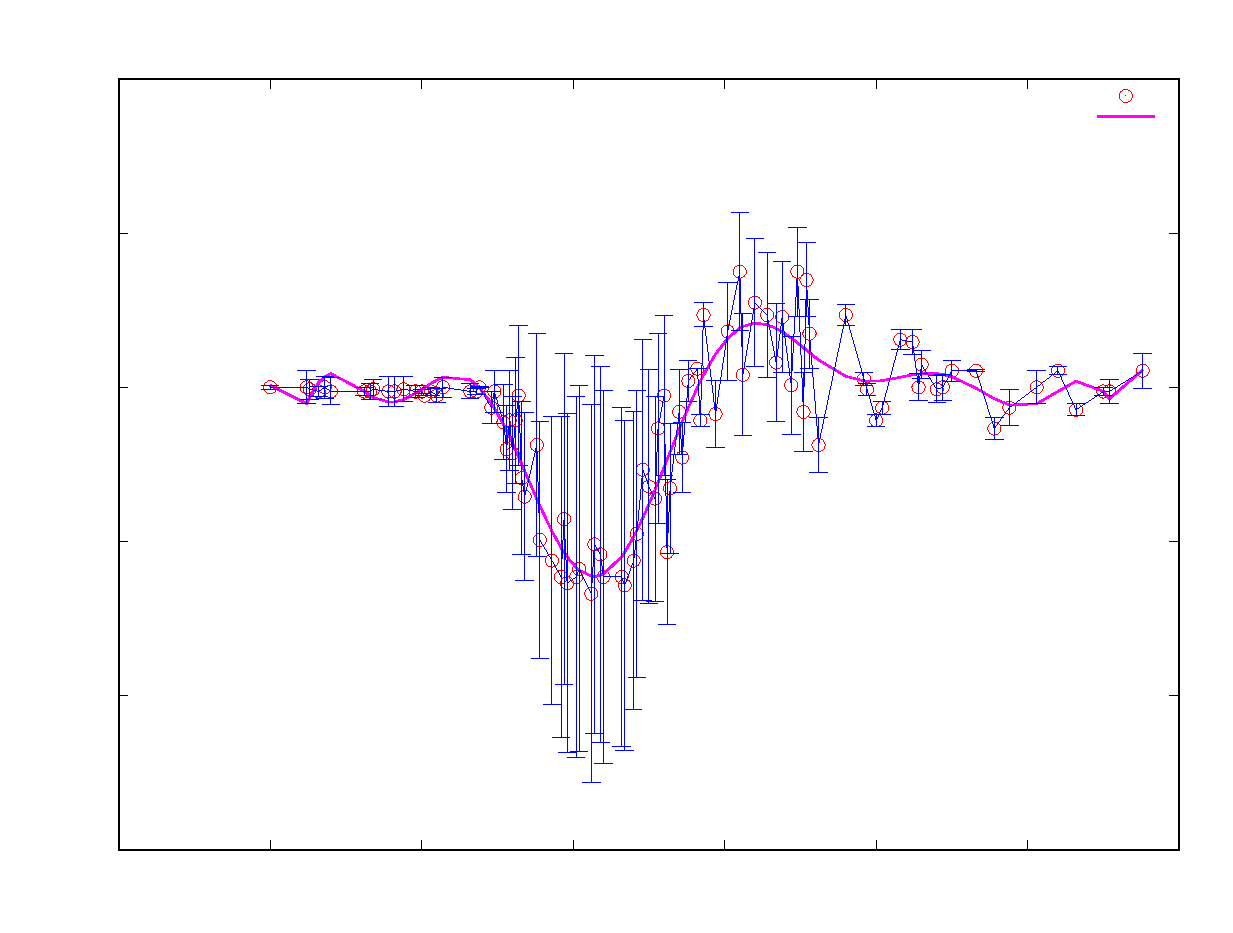
\includegraphics{poly}}%
    \gplfronttext
  \end{picture}%
\endgroup
}}
  \caption{Warmup: Polynomial Basis $n^{12}$}
\end{figure}

\subsection*{Bayesian Linear Regression}

Using Gaussian Likelihood and Prior, we solved for $W$ using Moore Penrose.
\begin{equation}
W_{ML} = (\Phi^T\Phi)^{-1}\Phi^Tt
\end{equation}

This was simple to implement, especially in Octave/Matlab. However, without normalization the error rate was close to the baseline linear basis and significantly worse than the polynomial.

\begin{figure}[h!] 
  \centering
  \scalebox{0.5}{{\large % GNUPLOT: LaTeX picture with Postscript
\begingroup
  \makeatletter
  \providecommand\color[2][]{%
    \GenericError{(gnuplot) \space\space\space\@spaces}{%
      Package color not loaded in conjunction with
      terminal option `colourtext'%
    }{See the gnuplot documentation for explanation.%
    }{Either use 'blacktext' in gnuplot or load the package
      color.sty in LaTeX.}%
    \renewcommand\color[2][]{}%
  }%
  \providecommand\includegraphics[2][]{%
    \GenericError{(gnuplot) \space\space\space\@spaces}{%
      Package graphicx or graphics not loaded%
    }{See the gnuplot documentation for explanation.%
    }{The gnuplot epslatex terminal needs graphicx.sty or graphics.sty.}%
    \renewcommand\includegraphics[2][]{}%
  }%
  \providecommand\rotatebox[2]{#2}%
  \@ifundefined{ifGPcolor}{%
    \newif\ifGPcolor
    \GPcolorfalse
  }{}%
  \@ifundefined{ifGPblacktext}{%
    \newif\ifGPblacktext
    \GPblacktexttrue
  }{}%
  % define a \g@addto@macro without @ in the name:
  \let\gplgaddtomacro\g@addto@macro
  % define empty templates for all commands taking text:
  \gdef\gplbacktext{}%
  \gdef\gplfronttext{}%
  \makeatother
  \ifGPblacktext
    % no textcolor at all
    \def\colorrgb#1{}%
    \def\colorgray#1{}%
  \else
    % gray or color?
    \ifGPcolor
      \def\colorrgb#1{\color[rgb]{#1}}%
      \def\colorgray#1{\color[gray]{#1}}%
      \expandafter\def\csname LTw\endcsname{\color{white}}%
      \expandafter\def\csname LTb\endcsname{\color{black}}%
      \expandafter\def\csname LTa\endcsname{\color{black}}%
      \expandafter\def\csname LT0\endcsname{\color[rgb]{1,0,0}}%
      \expandafter\def\csname LT1\endcsname{\color[rgb]{0,1,0}}%
      \expandafter\def\csname LT2\endcsname{\color[rgb]{0,0,1}}%
      \expandafter\def\csname LT3\endcsname{\color[rgb]{1,0,1}}%
      \expandafter\def\csname LT4\endcsname{\color[rgb]{0,1,1}}%
      \expandafter\def\csname LT5\endcsname{\color[rgb]{1,1,0}}%
      \expandafter\def\csname LT6\endcsname{\color[rgb]{0,0,0}}%
      \expandafter\def\csname LT7\endcsname{\color[rgb]{1,0.3,0}}%
      \expandafter\def\csname LT8\endcsname{\color[rgb]{0.5,0.5,0.5}}%
    \else
      % gray
      \def\colorrgb#1{\color{black}}%
      \def\colorgray#1{\color[gray]{#1}}%
      \expandafter\def\csname LTw\endcsname{\color{white}}%
      \expandafter\def\csname LTb\endcsname{\color{black}}%
      \expandafter\def\csname LTa\endcsname{\color{black}}%
      \expandafter\def\csname LT0\endcsname{\color{black}}%
      \expandafter\def\csname LT1\endcsname{\color{black}}%
      \expandafter\def\csname LT2\endcsname{\color{black}}%
      \expandafter\def\csname LT3\endcsname{\color{black}}%
      \expandafter\def\csname LT4\endcsname{\color{black}}%
      \expandafter\def\csname LT5\endcsname{\color{black}}%
      \expandafter\def\csname LT6\endcsname{\color{black}}%
      \expandafter\def\csname LT7\endcsname{\color{black}}%
      \expandafter\def\csname LT8\endcsname{\color{black}}%
    \fi
  \fi
  \setlength{\unitlength}{0.0500bp}%
  \begin{picture}(11520.00,8640.00)%
    \gplgaddtomacro\gplbacktext{%
      \colorrgb{0.00,0.00,0.00}%
      \put(860,640){\makebox(0,0)[r]{\strut{}-200}}%
      \colorrgb{0.00,0.00,0.00}%
      \put(860,1873){\makebox(0,0)[r]{\strut{}-150}}%
      \colorrgb{0.00,0.00,0.00}%
      \put(860,3106){\makebox(0,0)[r]{\strut{}-100}}%
      \colorrgb{0.00,0.00,0.00}%
      \put(860,4340){\makebox(0,0)[r]{\strut{}-50}}%
      \colorrgb{0.00,0.00,0.00}%
      \put(860,5573){\makebox(0,0)[r]{\strut{}0}}%
      \colorrgb{0.00,0.00,0.00}%
      \put(860,6806){\makebox(0,0)[r]{\strut{}50}}%
      \colorrgb{0.00,0.00,0.00}%
      \put(860,8039){\makebox(0,0)[r]{\strut{}100}}%
      \colorrgb{0.00,0.00,0.00}%
      \put(980,440){\makebox(0,0){\strut{}-10}}%
      \colorrgb{0.00,0.00,0.00}%
      \put(2434,440){\makebox(0,0){\strut{}0}}%
      \colorrgb{0.00,0.00,0.00}%
      \put(3888,440){\makebox(0,0){\strut{}10}}%
      \colorrgb{0.00,0.00,0.00}%
      \put(5342,440){\makebox(0,0){\strut{}20}}%
      \colorrgb{0.00,0.00,0.00}%
      \put(6797,440){\makebox(0,0){\strut{}30}}%
      \colorrgb{0.00,0.00,0.00}%
      \put(8251,440){\makebox(0,0){\strut{}40}}%
      \colorrgb{0.00,0.00,0.00}%
      \put(9705,440){\makebox(0,0){\strut{}50}}%
      \colorrgb{0.00,0.00,0.00}%
      \put(11159,440){\makebox(0,0){\strut{}60}}%
      \colorrgb{0.00,0.00,0.00}%
      \put(160,4339){\rotatebox{90}{\makebox(0,0){\strut{}force on head (g)}}}%
      \colorrgb{0.00,0.00,0.00}%
      \put(6069,140){\makebox(0,0){\strut{}time since impact(ms)}}%
      \csname LTb\endcsname%
      \put(6069,8339){\makebox(0,0){\strut{}Gaussian / Moore Penrose}}%
    }%
    \gplgaddtomacro\gplfronttext{%
      \csname LTb\endcsname%
      \put(10256,7876){\makebox(0,0)[r]{\strut{}Training Data}}%
      \csname LTb\endcsname%
      \put(10256,7676){\makebox(0,0)[r]{\strut{}Gaussian / Moore Penrose}}%
    }%
    \gplbacktext
    \put(0,0){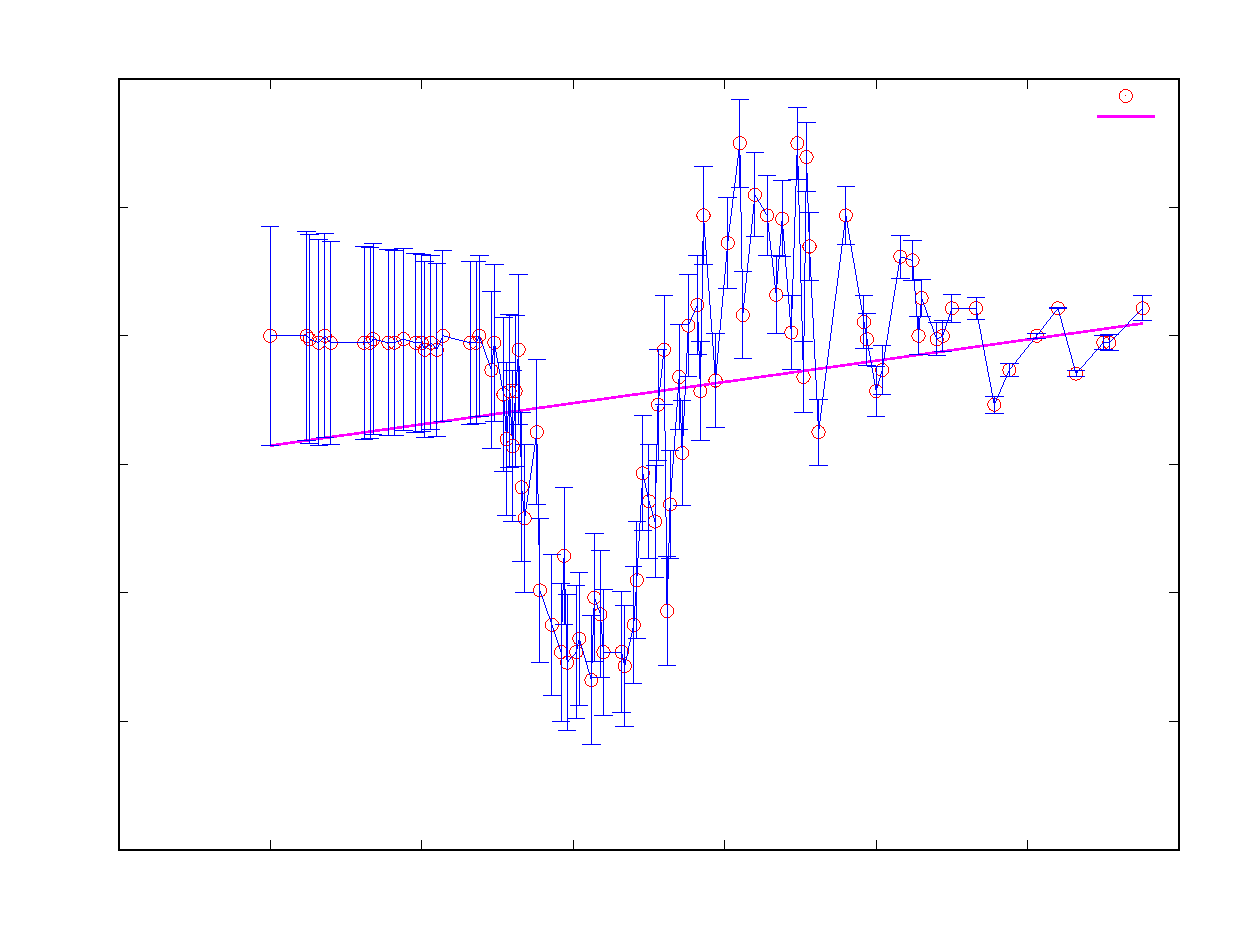
\includegraphics{gauss}}%
    \gplfronttext
  \end{picture}%
\endgroup
}}
  \caption{Warmup: Gaussian}
\end{figure}


\subsection*{Locally Weighted Linear Regression}

Locally Weighted Linear Regression (LWLR)\footnote{\emph{Machine Learning in Action} by Peter Harrington. \textsuperscript{\textcopyright} 2012 ISBN 978-1617290183} provided the lowest cost overall and a smooth fit to the data without overfitting given the profile of this dataset. A variety of $K$ values were attempted. 0.001 never converged. Values from 0.5, 1.0, 5.0 and 10.0 did converge with 1.0 seemingly providing the best balance between fit and smoothness.

LWLR is an expensive operation. Since the dataset here was small and did not match a typical straight line or polynomial pattern, it was appropriate to attempt LWLR.





\begin{figure}[h!] 
\centering
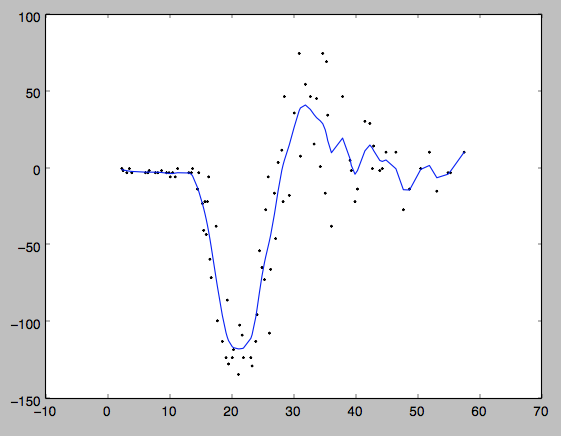
\includegraphics[scale=0.6]{lwlr}
\caption{Warmup: Locally Weighted Linear Regression $K=1$}
\end{figure}

\subsection*{Warmup Summary}
Across all basis functions, overall error rate was calculated by sum-of-squares:
\begin{equation}
J = \frac{1}{2N}\sum_{i=1}^N(y_i-t_i)^2
\end{equation}

The following table summarizes our results. LWLR was reasonably simple to implement and provided the lowest cost. For this particular data set, it would be our basis function of choice.

\begin{center}
    \begin{tabular}{| l | l |}
    \hline
    Basis & Lowest Error \\ \hline
    Linear Basis & \hfill 1293.0 \\
    Gaussian Basis & \hfill 1187.7 \\
    Polynomial Basis & \hfill 211.9 \\
    LWLR Basis & \hfill 185.6 \\
    \hline
    \end{tabular}
\end{center}


\section*{Predicting Movie Opening Weekend Revenues}


\subsection*{Preliminary Data Analysis}

The training set consists of movie metadata and textual movie reviews. From the sample code provided in the problem, the initial set of features has a classic problem of too many dimensions (105403) for too little data (1147).  This is mostly due to the unigrams converting each word of each movie review and description into a different dimension. Eliminating the unigrams as a first step significantly improved classification results and reduced dimensionality to only(!) 11276.

\subsection*{Subsection 2}

\section*{Conclusion}


\end{document}  
